%%%%%%%%%%%%%%%%%%%%%%%%%%%%%%%%%%%%%%%%%%%%%%%%%%%%%%%%%%%%
% 1.9 COMMUTATIVE ALGEBRA
% The Composition of Advanced Mathematics
%%%%%%%%%%%%%%%%%%%%%%%%%%%%%%%%%%%%%%%%%%%%%%%%%%%%%%%%%%%%

\section{Commutative Algebra}
\label{sec:commutative-algebra}

\prerequisite{
Ring theory from \cref{sec:ring-theory}, field theory from
\cref{sec:field-theory}, and module theory from \cref{sec:module-theory}.
}

\learningobjectives{
By the end of this section, the reader should be able to:
\begin{itemize}
    \item explain the role of commutative rings in algebra;
    \item work with ideals, prime ideals, and maximal ideals;
    \item interpret quotient rings through ideals;
    \item work with finitely generated ideals;
    \item define Noetherian rings and use the ascending chain condition;
    \item understand Hilbert's Basis Theorem;
    \item define radicals of ideals and radical ideals;
    \item work with nilpotent elements and nilradicals;
    \item define localization of rings and modules;
    \item understand localization at prime ideals;
    \item distinguish local rings from general rings;
    \item work with integral extensions and integral elements;
    \item understand the relationship between prime ideals and localization;
    \item define the spectrum of a commutative ring;
    \item understand chains of prime ideals and Krull dimension;
    \item recognize primary ideals and primary decomposition;
    \item explain how commutative algebra provides the algebraic foundation
    for algebraic geometry.
\end{itemize}
}

%%%%%%%%%%%%%%%%%%%%%%%%%%%%%%%%%%%%%%%%%%%%%%%%%%%%%%%%%%%%
\subsection{What Is Commutative Algebra?}
\label{subsec:what-is-commutative-algebra}
%%%%%%%%%%%%%%%%%%%%%%%%%%%%%%%%%%%%%%%%%%%%%%%%%%%%%%%%%%%%

Commutative algebra studies commutative rings, their ideals, their modules,
and the structural relationships among them.

A commutative ring \(R\) satisfies

\[ ab=ba \]

for every \(a,b\in R\).

Many familiar number systems and polynomial systems are commutative rings:

\[ \Z,\qquad \Q,\qquad \R,\qquad \C,\qquad F[x],\qquad F[x_1,\ldots,x_n]. \]

Commutative algebra is especially concerned with the structure of ideals and
prime ideals because they encode information about both algebra and geometry.

\begin{conceptbox}
Commutative algebra studies algebraic structures locally and globally through
rings, ideals, modules, localization, and prime ideals.

It provides much of the algebraic language underlying algebraic geometry and
algebraic number theory.
\end{conceptbox}

%%%%%%%%%%%%%%%%%%%%%%%%%%%%%%%%%%%%%%%%%%%%%%%%%%%%%%%%%%%%
\subsection{The Central Objects}
\label{subsec:commutative-algebra-central-objects}
%%%%%%%%%%%%%%%%%%%%%%%%%%%%%%%%%%%%%%%%%%%%%%%%%%%%%%%%%%%%

The main objects interact through a network of constructions.

\begin{center}
\begin{tikzpicture}[
    node distance=11mm and 16mm,
    box/.style={draw,rounded corners,align=center,inner sep=5pt},
    >=stealth
]
\node[box] (ring) {Commutative\\ring \(R\)};
\node[box,below left=of ring] (ideal) {Ideals\\\(I\trianglelefteq R\)};
\node[box,below right=of ring] (module) {\(R\)-modules};
\node[box,below=of ideal] (prime) {Prime and\\maximal ideals};
\node[box,below=of module] (loc) {Localization};
\node[box,below=22mm of ring] (geom) {Algebraic and geometric\\structure};

\draw[->,thick] (ring)--(ideal);
\draw[->,thick] (ring)--(module);
\draw[->,thick] (ideal)--(prime);
\draw[->,thick] (module)--(loc);
\draw[->,thick] (prime)--(geom);
\draw[->,thick] (loc)--(geom);
\end{tikzpicture}
\end{center}

%%%%%%%%%%%%%%%%%%%%%%%%%%%%%%%%%%%%%%%%%%%%%%%%%%%%%%%%%%%%
\subsection{Ideals Revisited}
\label{subsec:commutative-ideals}
%%%%%%%%%%%%%%%%%%%%%%%%%%%%%%%%%%%%%%%%%%%%%%%%%%%%%%%%%%%%

Ideals were introduced canonically in \cref{sec:ring-theory}. They become
central objects in commutative algebra.

\begin{definitionbox}{Ideal}
Let \(R\) be a commutative ring. A subset \(I\subseteq R\) is an
\emph{ideal} if:
\begin{enumerate}
    \item \(I\) is an additive subgroup of \(R\);
    \item for every \(r\in R\) and \(a\in I\),
    \[ ra\in I. \]
\end{enumerate}
\end{definitionbox}

Because multiplication is commutative,

\[ ra=ar, \]

so there is no distinction between left and right ideals.

%%%%%%%%%%%%%%%%%%%%%%%%%%%%%%%%%%%%%%%%%%%%%%%%%%%%%%%%%%%%
\subsection{Principal Ideals}
\label{subsec:commutative-principal-ideals}
%%%%%%%%%%%%%%%%%%%%%%%%%%%%%%%%%%%%%%%%%%%%%%%%%%%%%%%%%%%%

For \(a\in R\), the principal ideal generated by \(a\) is

\[ (a)=\{ra:r\in R\}. \]

The notation

\[ (a) \]

is read ``the ideal generated by \(a\).''

For example, in \(\Z\),

\[ (6)=6\Z=\{\ldots,-12,-6,0,6,12,\ldots\}. \]

%%%%%%%%%%%%%%%%%%%%%%%%%%%%%%%%%%%%%%%%%%%%%%%%%%%%%%%%%%%%
\subsection{Finitely Generated Ideals}
\label{subsec:finitely-generated-ideals}
%%%%%%%%%%%%%%%%%%%%%%%%%%%%%%%%%%%%%%%%%%%%%%%%%%%%%%%%%%%%

More generally, if

\[ a_1,\ldots,a_n\in R, \]

then the ideal generated by these elements is

\[ (a_1,\ldots,a_n)
=\{r_1a_1+\cdots+r_na_n:r_1,\ldots,r_n\in R\}. \]

\begin{definitionbox}{Finitely Generated Ideal}
An ideal \(I\trianglelefteq R\) is \emph{finitely generated} if there exist
\(a_1,\ldots,a_n\in R\) such that
\[ I=(a_1,\ldots,a_n). \]
\end{definitionbox}

%%%%%%%%%%%%%%%%%%%%%%%%%%%%%%%%%%%%%%%%%%%%%%%%%%%%%%%%%%%%
\subsection{Example: Ideals in the Integers}
\label{subsec:ideals-in-integers}
%%%%%%%%%%%%%%%%%%%%%%%%%%%%%%%%%%%%%%%%%%%%%%%%%%%%%%%%%%%%

Every ideal of \(\Z\) is principal.

For example,

\[ (12,18)=(6). \]

Indeed, every integer combination

\[ 12a+18b \]

is divisible by \(6\), and B\'ezout's identity gives integers \(a,b\) such
that

\[ 12a+18b=6. \]

Thus the ideal generated by \(12\) and \(18\) is exactly \(6\Z\).

%%%%%%%%%%%%%%%%%%%%%%%%%%%%%%%%%%%%%%%%%%%%%%%%%%%%%%%%%%%%
\subsection{Sums and Products of Ideals}
\label{subsec:sums-products-ideals}
%%%%%%%%%%%%%%%%%%%%%%%%%%%%%%%%%%%%%%%%%%%%%%%%%%%%%%%%%%%%

Let \(I,J\trianglelefteq R\).

Their sum is

\[ I+J=\{a+b:a\in I,\ b\in J\}. \]

Their product is the ideal

\[ IJ=\left\{\sum_{k=1}^{n}a_kb_k:a_k\in I,\ b_k\in J\right\}. \]

The product is generally not simply the set

\[ \{ab:a\in I,\ b\in J\}, \]

because sums of such products are required.

%%%%%%%%%%%%%%%%%%%%%%%%%%%%%%%%%%%%%%%%%%%%%%%%%%%%%%%%%%%%
\subsection{Ideal Containment}
\label{subsec:ideal-containment}
%%%%%%%%%%%%%%%%%%%%%%%%%%%%%%%%%%%%%%%%%%%%%%%%%%%%%%%%%%%%

Ideals are naturally organized by inclusion.

For example, in \(\Z\),

\[ (12)\subseteq(6)\subseteq(3)\subseteq(1)=\Z. \]

Notice the reversal between divisibility and ideal containment:

\[ a\mid b\quad\Longrightarrow\quad(b)\subseteq(a). \]

For instance,

\[ 3\mid12,\qquad(12)\subseteq(3). \]

\begin{center}
\begin{tikzpicture}[
    node distance=9mm,
    box/.style={draw,rounded corners,minimum width=20mm,inner sep=4pt},
    >=stealth
]
\node[box] (Z) {\(\Z\)};
\node[box,below=of Z] (3) {\((3)\)};
\node[box,below=of 3] (6) {\((6)\)};
\node[box,below=of 6] (12) {\((12)\)};
\node[below=of 12] (dots) {\(\vdots\)};

\draw[->] (12)--node[right]{\(\subseteq\)}(6);
\draw[->] (6)--node[right]{\(\subseteq\)}(3);
\draw[->] (3)--node[right]{\(\subseteq\)}(Z);
\end{tikzpicture}
\end{center}

%%%%%%%%%%%%%%%%%%%%%%%%%%%%%%%%%%%%%%%%%%%%%%%%%%%%%%%%%%%%
\subsection{Quotient Rings Revisited}
\label{subsec:commutative-quotient-rings}
%%%%%%%%%%%%%%%%%%%%%%%%%%%%%%%%%%%%%%%%%%%%%%%%%%%%%%%%%%%%

Given an ideal \(I\trianglelefteq R\), the quotient ring

\[ R/I \]

identifies elements whose difference belongs to \(I\).

Thus

\[ a+I=b+I \]

exactly when

\[ a-b\in I. \]

Quotient rings allow algebraic relations to be imposed by declaring elements
of \(I\) to be zero.

%%%%%%%%%%%%%%%%%%%%%%%%%%%%%%%%%%%%%%%%%%%%%%%%%%%%%%%%%%%%
\subsection{Prime Ideals}
\label{subsec:prime-ideals}
%%%%%%%%%%%%%%%%%%%%%%%%%%%%%%%%%%%%%%%%%%%%%%%%%%%%%%%%%%%%

Prime ideals play a role analogous to prime numbers.

\begin{definitionbox}{Prime Ideal}
Let \(R\) be a commutative ring with identity. A proper ideal
\(\mathfrak p\subsetneq R\) is \emph{prime} if
\[ ab\in\mathfrak p\implies a\in\mathfrak p\text{ or }b\in\mathfrak p. \]
\end{definitionbox}

The symbol

\[ \mathfrak p \]

is a lowercase Fraktur \(p\), commonly used for prime ideals, and is read
``fraktur \(p\)'' or simply ``\(p\)'' when the context is clear.

%%%%%%%%%%%%%%%%%%%%%%%%%%%%%%%%%%%%%%%%%%%%%%%%%%%%%%%%%%%%
\subsection{Prime Ideals and Integral Domains}
\label{subsec:prime-ideal-domain}
%%%%%%%%%%%%%%%%%%%%%%%%%%%%%%%%%%%%%%%%%%%%%%%%%%%%%%%%%%%%

Prime ideals can be characterized using quotient rings.

\begin{theorem}
Let \(R\) be a commutative ring with identity and
\(\mathfrak p\subsetneq R\). Then
\[ \mathfrak p\text{ is prime}
\iff
R/\mathfrak p\text{ is an integral domain}. \]
\end{theorem}

\begin{proof}
Suppose \(\mathfrak p\) is prime. If

\[ (a+\mathfrak p)(b+\mathfrak p)=\mathfrak p, \]

then

\[ ab\in\mathfrak p. \]

Since \(\mathfrak p\) is prime,

\[ a\in\mathfrak p\quad\text{or}\quad b\in\mathfrak p. \]

Hence

\[ a+\mathfrak p=\mathfrak p\quad\text{or}\quad b+\mathfrak p=\mathfrak p. \]

Therefore \(R/\mathfrak p\) has no zero divisors.

Conversely, suppose \(R/\mathfrak p\) is an integral domain and

\[ ab\in\mathfrak p. \]

Then

\[ (a+\mathfrak p)(b+\mathfrak p)=\mathfrak p. \]

Since the quotient has no zero divisors,

\[ a+\mathfrak p=\mathfrak p\quad\text{or}\quad b+\mathfrak p=\mathfrak p, \]

so

\[ a\in\mathfrak p\quad\text{or}\quad b\in\mathfrak p. \]

Thus \(\mathfrak p\) is prime.
\end{proof}

%%%%%%%%%%%%%%%%%%%%%%%%%%%%%%%%%%%%%%%%%%%%%%%%%%%%%%%%%%%%
\subsection{Maximal Ideals}
\label{subsec:maximal-ideals}
%%%%%%%%%%%%%%%%%%%%%%%%%%%%%%%%%%%%%%%%%%%%%%%%%%%%%%%%%%%%

\begin{definitionbox}{Maximal Ideal}
A proper ideal \(\mathfrak m\subsetneq R\) is \emph{maximal} if there is no
ideal \(I\) satisfying
\[ \mathfrak m\subsetneq I\subsetneq R. \]
\end{definitionbox}

The notation

\[ \mathfrak m \]

is a lowercase Fraktur \(m\), commonly used for maximal ideals.

%%%%%%%%%%%%%%%%%%%%%%%%%%%%%%%%%%%%%%%%%%%%%%%%%%%%%%%%%%%%
\subsection{Maximal Ideals and Fields}
\label{subsec:maximal-ideal-field}
%%%%%%%%%%%%%%%%%%%%%%%%%%%%%%%%%%%%%%%%%%%%%%%%%%%%%%%%%%%%

\begin{theorem}
Let \(R\) be a commutative ring with identity. Then
\[ \mathfrak m\text{ is maximal}
\iff
R/\mathfrak m\text{ is a field}. \]
\end{theorem}

Consequently,

\[ \boxed{\text{maximal ideal}\Longrightarrow\text{prime ideal}.} \]

The converse is not generally true.

%%%%%%%%%%%%%%%%%%%%%%%%%%%%%%%%%%%%%%%%%%%%%%%%%%%%%%%%%%%%
\subsection{Prime and Maximal Ideals in \(\Z\)}
\label{subsec:prime-maximal-z}
%%%%%%%%%%%%%%%%%%%%%%%%%%%%%%%%%%%%%%%%%%%%%%%%%%%%%%%%%%%%

Every ideal of \(\Z\) has the form

\[ (n). \]

If \(p\) is prime, then

\[ \Z/(p) \]

is a field.

Therefore,

\[ (p) \]

is maximal and prime.

The zero ideal

\[ (0) \]

is also prime because

\[ \Z/(0)\cong\Z \]

is an integral domain.

However, \((0)\) is not maximal because \(\Z\) is not a field.

%%%%%%%%%%%%%%%%%%%%%%%%%%%%%%%%%%%%%%%%%%%%%%%%%%%%%%%%%%%%
\subsection{Visualizing Prime and Maximal Ideals}
\label{subsec:prime-maximal-visual}
%%%%%%%%%%%%%%%%%%%%%%%%%%%%%%%%%%%%%%%%%%%%%%%%%%%%%%%%%%%%

\begin{center}
\begin{tikzpicture}[
    node distance=11mm,
    box/.style={draw,rounded corners,align=center,inner sep=5pt},
    >=stealth
]
\node[box] (proper) {Proper ideals};
\node[box,below=of proper] (prime) {Prime ideals\\\(R/\mathfrak p\) is a domain};
\node[box,below=of prime] (max) {Maximal ideals\\\(R/\mathfrak m\) is a field};

\draw[->,thick] (max)--node[right]{always}(prime);
\draw[->,thick] (prime)--(proper);
\end{tikzpicture}
\end{center}

Every maximal ideal is prime, but a prime ideal need not be maximal.

%%%%%%%%%%%%%%%%%%%%%%%%%%%%%%%%%%%%%%%%%%%%%%%%%%%%%%%%%%%%
\subsection{Worked Example: Prime and Maximal Ideals}
\label{subsec:worked-prime-maximal}
%%%%%%%%%%%%%%%%%%%%%%%%%%%%%%%%%%%%%%%%%%%%%%%%%%%%%%%%%%%%

\begin{workedexamplebox}{Classifying Ideals in \(\Z\)}

Determine whether \((5)\) and \((6)\) are prime or maximal ideals of \(\Z\).

\begin{tabularx}{\textwidth}{@{}>{\raggedright\arraybackslash}p{0.42\textwidth}X@{}}
Examine \(\Z/(5)\). & \(\Z/5\Z\) is a field.\\
Classify \((5)\). & \((5)\) is maximal and therefore prime.\\
Examine \(\Z/(6)\). & \(\Z/6\Z\) has zero divisors since \([2][3]=[0]\).\\
Classify \((6)\). & \((6)\) is neither prime nor maximal.
\end{tabularx}

\begin{answerbox}
\[ (5)\text{ is maximal and prime},\qquad(6)\text{ is neither}. \]
\end{answerbox}
\end{workedexamplebox}

%%%%%%%%%%%%%%%%%%%%%%%%%%%%%%%%%%%%%%%%%%%%%%%%%%%%%%%%%%%%
\subsection{The Radical of an Ideal}
\label{subsec:radical-of-ideal}
%%%%%%%%%%%%%%%%%%%%%%%%%%%%%%%%%%%%%%%%%%%%%%%%%%%%%%%%%%%%

\begin{definitionbox}{Radical of an Ideal}
Let \(I\trianglelefteq R\). The \emph{radical} of \(I\) is
\[ \sqrt{I}=\{r\in R:r^n\in I\text{ for some integer }n\geq1\}. \]
\end{definitionbox}

The notation

\[ \sqrt{I} \]

is read ``the radical of \(I\).''

Although it resembles square-root notation, it represents an ideal rather
than an ordinary numerical square root.

%%%%%%%%%%%%%%%%%%%%%%%%%%%%%%%%%%%%%%%%%%%%%%%%%%%%%%%%%%%%
\subsection{Example of an Ideal Radical}
\label{subsec:ideal-radical-example}
%%%%%%%%%%%%%%%%%%%%%%%%%%%%%%%%%%%%%%%%%%%%%%%%%%%%%%%%%%%%

Consider

\[ I=(12)\subseteq\Z. \]

An integer belongs to \(\sqrt{(12)}\) if some positive power of it is
divisible by \(12\).

Since

\[ 12=2^2\cdot3, \]

an integer must contain both prime factors \(2\) and \(3\).

Therefore,

\[ \sqrt{(12)}=(6). \]

%%%%%%%%%%%%%%%%%%%%%%%%%%%%%%%%%%%%%%%%%%%%%%%%%%%%%%%%%%%%
\subsection{Radical Ideals}
\label{subsec:radical-ideals}
%%%%%%%%%%%%%%%%%%%%%%%%%%%%%%%%%%%%%%%%%%%%%%%%%%%%%%%%%%%%

\begin{definitionbox}{Radical Ideal}
An ideal \(I\trianglelefteq R\) is \emph{radical} if
\[ \sqrt{I}=I. \]
\end{definitionbox}

Equivalently,

\[ r^n\in I\implies r\in I. \]

Every prime ideal is radical.

%%%%%%%%%%%%%%%%%%%%%%%%%%%%%%%%%%%%%%%%%%%%%%%%%%%%%%%%%%%%
\subsection{Nilpotent Elements}
\label{subsec:nilpotent-elements}
%%%%%%%%%%%%%%%%%%%%%%%%%%%%%%%%%%%%%%%%%%%%%%%%%%%%%%%%%%%%

\begin{definitionbox}{Nilpotent Element}
An element \(a\in R\) is \emph{nilpotent} if
\[ a^n=0 \]
for some positive integer \(n\).
\end{definitionbox}

For example, in

\[ \Z/8\Z, \]

the element \([2]\) is not nilpotent because its powers do not become zero,
but \([4]\) is nilpotent since

\[ [4]^2=[16]=[0]. \]

%%%%%%%%%%%%%%%%%%%%%%%%%%%%%%%%%%%%%%%%%%%%%%%%%%%%%%%%%%%%
\subsection{The Nilradical}
\label{subsec:nilradical}
%%%%%%%%%%%%%%%%%%%%%%%%%%%%%%%%%%%%%%%%%%%%%%%%%%%%%%%%%%%%

The set of all nilpotent elements of \(R\) is called the
\emph{nilradical}.

It is denoted

\[ \sqrt{(0)}. \]

Thus

\[ \sqrt{(0)}=\{r\in R:r^n=0\text{ for some }n\geq1\}. \]

A fundamental theorem gives another characterization.

\begin{theorem}
For a commutative ring \(R\),
\[ \sqrt{(0)}=\bigcap_{\mathfrak p\in\Spec(R)}\mathfrak p. \]
\end{theorem}

Thus the nilradical is the intersection of all prime ideals.

%%%%%%%%%%%%%%%%%%%%%%%%%%%%%%%%%%%%%%%%%%%%%%%%%%%%%%%%%%%%
\subsection{Reduced Rings}
\label{subsec:reduced-rings}
%%%%%%%%%%%%%%%%%%%%%%%%%%%%%%%%%%%%%%%%%%%%%%%%%%%%%%%%%%%%

\begin{definitionbox}{Reduced Ring}
A commutative ring \(R\) is \emph{reduced} if it has no nonzero nilpotent
elements.
\end{definitionbox}

Equivalently,

\[ \sqrt{(0)}=(0). \]

Every integral domain is reduced, but a reduced ring need not be an integral
domain.

%%%%%%%%%%%%%%%%%%%%%%%%%%%%%%%%%%%%%%%%%%%%%%%%%%%%%%%%%%%%
\subsection{Noetherian Rings}
\label{subsec:noetherian-rings}
%%%%%%%%%%%%%%%%%%%%%%%%%%%%%%%%%%%%%%%%%%%%%%%%%%%%%%%%%%%%

The Noetherian condition prevents ideals from becoming infinitely more
complicated through an endless strictly increasing chain.

\begin{definitionbox}{Noetherian Ring}
A commutative ring \(R\) is \emph{Noetherian} if every ideal of \(R\) is
finitely generated.
\end{definitionbox}

Equivalently, \(R\) is Noetherian if every ascending chain

\[ I_1\subseteq I_2\subseteq I_3\subseteq\cdots \]

eventually stabilizes.

%%%%%%%%%%%%%%%%%%%%%%%%%%%%%%%%%%%%%%%%%%%%%%%%%%%%%%%%%%%%
\subsection{Ascending Chain Condition}
\label{subsec:acc-ideals}
%%%%%%%%%%%%%%%%%%%%%%%%%%%%%%%%%%%%%%%%%%%%%%%%%%%%%%%%%%%%

The chain

\[ I_1\subseteq I_2\subseteq I_3\subseteq\cdots \]

stabilizes if there exists some \(N\) such that

\[ I_N=I_{N+1}=I_{N+2}=\cdots. \]

\begin{center}
\begin{tikzpicture}[
    node distance=8mm,
    every node/.style={font=\small},
    >=stealth
]
\node (I1) {\(I_1\)};
\node[right=of I1] (I2) {\(I_2\)};
\node[right=of I2] (I3) {\(I_3\)};
\node[right=of I3] (IN) {\(I_N\)};
\node[right=of IN] (IN2) {\(I_N\)};
\node[right=of IN2] (dots) {\(\cdots\)};

\draw[->] (I1)--node[above]{\(\subseteq\)}(I2);
\draw[->] (I2)--node[above]{\(\subseteq\)}(I3);
\draw[->,dashed] (I3)--(IN);
\draw[->] (IN)--node[above]{\(=\)}(IN2);
\draw[->] (IN2)--node[above]{\(=\)}(dots);
\end{tikzpicture}
\end{center}

This is the \emph{ascending chain condition}, abbreviated ACC.

%%%%%%%%%%%%%%%%%%%%%%%%%%%%%%%%%%%%%%%%%%%%%%%%%%%%%%%%%%%%
\subsection{Why Finite Generation and ACC Are Equivalent}
\label{subsec:noetherian-equivalence}
%%%%%%%%%%%%%%%%%%%%%%%%%%%%%%%%%%%%%%%%%%%%%%%%%%%%%%%%%%%%

Suppose every ideal is finitely generated and

\[ I_1\subseteq I_2\subseteq\cdots. \]

Let

\[ I=\bigcup_{n=1}^{\infty}I_n. \]

The union is an ideal because the ideals form an ascending chain.

Since \(I\) is finitely generated,

\[ I=(a_1,\ldots,a_k). \]

All generators eventually belong to some common \(I_N\). Therefore,

\[ I=I_N, \]

and the chain stabilizes.

Conversely, if every ascending chain stabilizes, repeatedly adding generators
to a non-finitely-generated ideal would produce a strictly increasing
infinite chain, which is impossible.

%%%%%%%%%%%%%%%%%%%%%%%%%%%%%%%%%%%%%%%%%%%%%%%%%%%%%%%%%%%%
\subsection{Examples of Noetherian Rings}
\label{subsec:noetherian-examples}
%%%%%%%%%%%%%%%%%%%%%%%%%%%%%%%%%%%%%%%%%%%%%%%%%%%%%%%%%%%%

Every field is Noetherian because its only ideals are

\[ (0)\qquad\text{and}\qquad F. \]

Every principal ideal domain is Noetherian because every ideal is generated
by one element.

Therefore,

\[ \Z \]

is Noetherian.

A major theorem shows that polynomial rings over Noetherian rings remain
Noetherian.

%%%%%%%%%%%%%%%%%%%%%%%%%%%%%%%%%%%%%%%%%%%%%%%%%%%%%%%%%%%%
\subsection{Hilbert's Basis Theorem}
\label{subsec:hilbert-basis-theorem}
%%%%%%%%%%%%%%%%%%%%%%%%%%%%%%%%%%%%%%%%%%%%%%%%%%%%%%%%%%%%

\begin{theorem}[Hilbert's Basis Theorem]
If \(R\) is a Noetherian commutative ring, then
\[ R[x] \]
is Noetherian.
\end{theorem}

Repeated application gives

\[ R[x_1,\ldots,x_n] \]

Noetherian whenever \(R\) is Noetherian.

In particular, if \(F\) is a field, then

\[ F[x_1,\ldots,x_n] \]

is Noetherian.

\begin{importantbox}
Hilbert's Basis Theorem guarantees that every ideal in a polynomial ring
\[ F[x_1,\ldots,x_n] \]
is finitely generated, even though the ring contains infinitely many
polynomials.
\end{importantbox}

%%%%%%%%%%%%%%%%%%%%%%%%%%%%%%%%%%%%%%%%%%%%%%%%%%%%%%%%%%%%
\subsection{Why Hilbert's Basis Theorem Matters}
\label{subsec:why-hilbert-basis-matters}
%%%%%%%%%%%%%%%%%%%%%%%%%%%%%%%%%%%%%%%%%%%%%%%%%%%%%%%%%%%%

Suppose

\[ I\trianglelefteq F[x_1,\ldots,x_n]. \]

Hilbert's Basis Theorem guarantees the existence of finitely many
polynomials

\[ f_1,\ldots,f_k \]

such that

\[ I=(f_1,\ldots,f_k). \]

Thus an ideal containing infinitely many polynomials can still be completely
determined by finite algebraic data.

\begin{center}
\begin{tikzpicture}[
    node distance=11mm,
    box/.style={draw,rounded corners,align=center,inner sep=5pt},
    >=stealth
]
\node[box] (infinite) {Potentially infinitely many\\polynomials in \(I\)};
\node[box,below=of infinite] (finite) {Finite generators\\\(f_1,\ldots,f_k\)};
\node[box,below=of finite] (ideal) {\(I=(f_1,\ldots,f_k)\)};

\draw[->,thick] (infinite)--node[right]{Noetherian}(finite);
\draw[->,thick] (finite)--(ideal);
\end{tikzpicture}
\end{center}

%%%%%%%%%%%%%%%%%%%%%%%%%%%%%%%%%%%%%%%%%%%%%%%%%%%%%%%%%%%%
\subsection{Multiplicatively Closed Sets}
\label{subsec:multiplicatively-closed-sets}
%%%%%%%%%%%%%%%%%%%%%%%%%%%%%%%%%%%%%%%%%%%%%%%%%%%%%%%%%%%%

Localization requires a collection of elements that will become invertible.

\begin{definitionbox}{Multiplicatively Closed Set}
A subset \(S\subseteq R\) is \emph{multiplicatively closed} if
\[ 1\in S \]
and
\[ a,b\in S\implies ab\in S. \]
\end{definitionbox}

Usually one also requires

\[ 0\notin S \]

when constructing a nonzero localization.

%%%%%%%%%%%%%%%%%%%%%%%%%%%%%%%%%%%%%%%%%%%%%%%%%%%%%%%%%%%%
\subsection{Localization of a Ring}
\label{subsec:localization-ring}
%%%%%%%%%%%%%%%%%%%%%%%%%%%%%%%%%%%%%%%%%%%%%%%%%%%%%%%%%%%%

Localization generalizes the construction of fractions.

\begin{definitionbox}{Localization}
Let \(R\) be a commutative ring and \(S\subseteq R\) a multiplicatively
closed set. The \emph{localization} of \(R\) at \(S\), denoted
\[ S^{-1}R, \]
consists of fractions
\[ \frac{r}{s},\qquad r\in R,\quad s\in S, \]
under an appropriate equivalence relation.
\end{definitionbox}

The notation

\[ S^{-1}R \]

is read ``\(S\) inverse \(R\)'' or, more naturally, ``the localization of
\(R\) at \(S\).''

Every element of \(S\) becomes invertible in \(S^{-1}R\).

%%%%%%%%%%%%%%%%%%%%%%%%%%%%%%%%%%%%%%%%%%%%%%%%%%%%%%%%%%%%
\subsection{From Integers to Rational Numbers}
\label{subsec:localization-z-q}
%%%%%%%%%%%%%%%%%%%%%%%%%%%%%%%%%%%%%%%%%%%%%%%%%%%%%%%%%%%%

Take

\[ R=\Z,\qquad S=\Z\setminus\{0\}. \]

Then

\[ S^{-1}\Z\cong\Q. \]

Thus the rational numbers arise by making every nonzero integer invertible.

\begin{center}
\begin{tikzpicture}[
    node distance=20mm,
    box/.style={draw,rounded corners,align=center,inner sep=6pt},
    >=stealth
]
\node[box] (Z) {\(\Z\)};
\node[box,right=of Z] (Q) {\(\Q\)};
\draw[->,thick] (Z)--node[above]{invert all \(n\neq0\)}
node[below]{localization}(Q);
\end{tikzpicture}
\end{center}

Localization extends this familiar fraction construction to arbitrary
commutative rings.

%%%%%%%%%%%%%%%%%%%%%%%%%%%%%%%%%%%%%%%%%%%%%%%%%%%%%%%%%%%%
\subsection{Equality in a Localization}
\label{subsec:equality-localization}
%%%%%%%%%%%%%%%%%%%%%%%%%%%%%%%%%%%%%%%%%%%%%%%%%%%%%%%%%%%%

When \(R\) is an integral domain, the familiar rule applies:

\[ \frac{a}{s}=\frac{b}{t}\iff at=bs. \]

For rings with zero divisors, the general equivalence relation is more
subtle.

One defines

\[ \frac{a}{s}=\frac{b}{t} \]

if there exists \(u\in S\) such that

\[ u(at-bs)=0. \]

This adjustment is necessary because cancellation may fail in rings with
zero divisors.

%%%%%%%%%%%%%%%%%%%%%%%%%%%%%%%%%%%%%%%%%%%%%%%%%%%%%%%%%%%%
\subsection{Arithmetic in a Localization}
\label{subsec:localization-arithmetic}
%%%%%%%%%%%%%%%%%%%%%%%%%%%%%%%%%%%%%%%%%%%%%%%%%%%%%%%%%%%%

Addition and multiplication resemble ordinary fractions:

\[ \frac{a}{s}+\frac{b}{t}=\frac{at+bs}{st}, \]

and

\[ \frac{a}{s}\frac{b}{t}=\frac{ab}{st}. \]

The canonical ring homomorphism is

\[ \iota:R\to S^{-1}R,\qquad \iota(r)=\frac{r}{1}. \]

%%%%%%%%%%%%%%%%%%%%%%%%%%%%%%%%%%%%%%%%%%%%%%%%%%%%%%%%%%%%
\subsection{Localization at a Prime Ideal}
\label{subsec:localization-prime}
%%%%%%%%%%%%%%%%%%%%%%%%%%%%%%%%%%%%%%%%%%%%%%%%%%%%%%%%%%%%

Let \(\mathfrak p\) be a prime ideal.

The complement

\[ S=R\setminus\mathfrak p \]

is multiplicatively closed.

The localization

\[ R_{\mathfrak p}=S^{-1}R \]

is called the \emph{localization of \(R\) at \(\mathfrak p\)}.

The notation

\[ R_{\mathfrak p} \]

is read ``\(R\) localized at \(\mathfrak p\).''

%%%%%%%%%%%%%%%%%%%%%%%%%%%%%%%%%%%%%%%%%%%%%%%%%%%%%%%%%%%%
\subsection{What Localization at a Prime Does}
\label{subsec:meaning-localization-prime}
%%%%%%%%%%%%%%%%%%%%%%%%%%%%%%%%%%%%%%%%%%%%%%%%%%%%%%%%%%%%

In

\[ R_{\mathfrak p}, \]

every element outside \(\mathfrak p\) becomes invertible.

Thus the localization focuses attention on the algebraic behavior associated
with the prime ideal \(\mathfrak p\).

\begin{center}
\begin{tikzpicture}[
    node distance=12mm,
    box/.style={draw,rounded corners,align=center,inner sep=5pt},
    >=stealth
]
\node[box] (R) {Global ring\\\(R\)};
\node[box,below left=of R] (outside) {Elements outside\\\(\mathfrak p\)};
\node[box,below right=of R] (inside) {Behavior near\\\(\mathfrak p\)};
\node[box,below=22mm of R] (Rp) {Local ring\\\(R_{\mathfrak p}\)};

\draw[->,thick] (R)--(outside);
\draw[->,thick] (R)--(inside);
\draw[->,thick] (outside)--node[left]{make invertible}(Rp);
\draw[->,thick] (inside)--(Rp);
\end{tikzpicture}
\end{center}

This global-to-local transition is one of the defining ideas of commutative
algebra.

%%%%%%%%%%%%%%%%%%%%%%%%%%%%%%%%%%%%%%%%%%%%%%%%%%%%%%%%%%%%
\subsection{Local Rings}
\label{subsec:local-rings}
%%%%%%%%%%%%%%%%%%%%%%%%%%%%%%%%%%%%%%%%%%%%%%%%%%%%%%%%%%%%

\begin{definitionbox}{Local Ring}
A commutative ring \(R\) is called a \emph{local ring} if it has exactly one
maximal ideal.
\end{definitionbox}

If the unique maximal ideal is \(\mathfrak m\), one often refers to

\[ (R,\mathfrak m) \]

as a local ring.

%%%%%%%%%%%%%%%%%%%%%%%%%%%%%%%%%%%%%%%%%%%%%%%%%%%%%%%%%%%%
\subsection{Units in a Local Ring}
\label{subsec:units-local-ring}
%%%%%%%%%%%%%%%%%%%%%%%%%%%%%%%%%%%%%%%%%%%%%%%%%%%%%%%%%%%%

A useful characterization is:

\begin{theorem}
Let \((R,\mathfrak m)\) be a local ring. Then
\[ R^\times=R\setminus\mathfrak m, \]
where \(R^\times\) denotes the set of units of \(R\).
\end{theorem}

Thus every element outside the unique maximal ideal is invertible.

Conversely, every nonunit lies inside the maximal ideal.

%%%%%%%%%%%%%%%%%%%%%%%%%%%%%%%%%%%%%%%%%%%%%%%%%%%%%%%%%%%%
\subsection{Localization Produces Local Rings}
\label{subsec:localization-produces-local-rings}
%%%%%%%%%%%%%%%%%%%%%%%%%%%%%%%%%%%%%%%%%%%%%%%%%%%%%%%%%%%%

If \(\mathfrak p\) is a prime ideal of \(R\), then

\[ R_{\mathfrak p} \]

is a local ring.

Its unique maximal ideal is

\[ \mathfrak pR_{\mathfrak p}. \]

Therefore localization provides a systematic way to construct local rings.

%%%%%%%%%%%%%%%%%%%%%%%%%%%%%%%%%%%%%%%%%%%%%%%%%%%%%%%%%%%%
\subsection{Example: Localizing the Integers}
\label{subsec:localizing-integers-prime}
%%%%%%%%%%%%%%%%%%%%%%%%%%%%%%%%%%%%%%%%%%%%%%%%%%%%%%%%%%%%

Let \(p\) be prime.

Then

\[ \Z_{(p)}=\left\{\frac{a}{b}\in\Q:p\nmid b\right\}. \]

Only denominators not divisible by \(p\) are allowed.

For example,

\[ \frac{1}{2}\in\Z_{(3)}, \]

but

\[ \frac{1}{3}\notin\Z_{(3)}. \]

The unique maximal ideal is

\[ p\Z_{(p)}. \]

%%%%%%%%%%%%%%%%%%%%%%%%%%%%%%%%%%%%%%%%%%%%%%%%%%%%%%%%%%%%
\subsection{Localization of Modules}
\label{subsec:localization-modules}
%%%%%%%%%%%%%%%%%%%%%%%%%%%%%%%%%%%%%%%%%%%%%%%%%%%%%%%%%%%%

Localization also applies to modules.

Let \(M\) be an \(R\)-module and \(S\subseteq R\) multiplicatively closed.

The localization

\[ S^{-1}M \]

consists of fractions

\[ \frac{m}{s},\qquad m\in M,\quad s\in S. \]

It naturally becomes an \(S^{-1}R\)-module.

%%%%%%%%%%%%%%%%%%%%%%%%%%%%%%%%%%%%%%%%%%%%%%%%%%%%%%%%%%%%
\subsection{Why Localize Modules?}
\label{subsec:why-localize-modules}
%%%%%%%%%%%%%%%%%%%%%%%%%%%%%%%%%%%%%%%%%%%%%%%%%%%%%%%%%%%%

Localization allows a module to be examined near a chosen prime ideal.

For

\[ \mathfrak p\in\Spec(R), \]

one writes

\[ M_{\mathfrak p}=(R\setminus\mathfrak p)^{-1}M. \]

Properties of \(M\) can often be understood by studying all localizations

\[ M_{\mathfrak p}. \]

This leads to the powerful principle that many algebraic questions are
\emph{local}.

%%%%%%%%%%%%%%%%%%%%%%%%%%%%%%%%%%%%%%%%%%%%%%%%%%%%%%%%%%%%
\subsection{Local-to-Global Thinking}
\label{subsec:local-global-thinking}
%%%%%%%%%%%%%%%%%%%%%%%%%%%%%%%%%%%%%%%%%%%%%%%%%%%%%%%%%%%%

Commutative algebra repeatedly moves between global and local information.

\begin{center}
\begin{tikzpicture}[
    node distance=23mm,
    box/.style={draw,rounded corners,align=center,inner sep=6pt},
    >=stealth
]
\node[box] (global) {Global object\\\(R\) or \(M\)};
\node[box,right=of global] (local) {Local objects\\\(R_{\mathfrak p}\), \(M_{\mathfrak p}\)};

\draw[->,thick,bend left=18] (global) to node[above]{localize}(local);
\draw[->,thick,bend left=18] (local) to node[below]{assemble information}(global);
\end{tikzpicture}
\end{center}

Rather than studying a complicated ring everywhere at once, localization
allows one to isolate behavior around individual prime ideals.

%%%%%%%%%%%%%%%%%%%%%%%%%%%%%%%%%%%%%%%%%%%%%%%%%%%%%%%%%%%%
\subsection{Integral Elements}
\label{subsec:integral-elements}
%%%%%%%%%%%%%%%%%%%%%%%%%%%%%%%%%%%%%%%%%%%%%%%%%%%%%%%%%%%%

Suppose

\[ R\subseteq S \]

are commutative rings.

\begin{definitionbox}{Integral Element}
An element \(s\in S\) is \emph{integral over \(R\)} if it satisfies a monic
polynomial equation
\[ s^n+a_{n-1}s^{n-1}+\cdots+a_1s+a_0=0 \]
with
\[ a_0,\ldots,a_{n-1}\in R. \]
\end{definitionbox}

A polynomial is \emph{monic} when its leading coefficient is \(1\).

%%%%%%%%%%%%%%%%%%%%%%%%%%%%%%%%%%%%%%%%%%%%%%%%%%%%%%%%%%%%
\subsection{Example of an Integral Element}
\label{subsec:integral-element-example}
%%%%%%%%%%%%%%%%%%%%%%%%%%%%%%%%%%%%%%%%%%%%%%%%%%%%%%%%%%%%

Consider

\[ \sqrt{2}\in\R. \]

It satisfies

\[ x^2-2=0. \]

Since

\[ x^2-2\in\Z[x] \]

is monic,

\[ \sqrt{2} \]

is integral over \(\Z\).

More generally, every algebraic integer is integral over \(\Z\).

%%%%%%%%%%%%%%%%%%%%%%%%%%%%%%%%%%%%%%%%%%%%%%%%%%%%%%%%%%%%
\subsection{Integral Extensions}
\label{subsec:integral-extensions}
%%%%%%%%%%%%%%%%%%%%%%%%%%%%%%%%%%%%%%%%%%%%%%%%%%%%%%%%%%%%

\begin{definitionbox}{Integral Extension}
A ring extension
\[ R\subseteq S \]
is \emph{integral} if every element of \(S\) is integral over \(R\).
\end{definitionbox}

Integral extensions generalize algebraic field extensions to the setting of
commutative rings.

%%%%%%%%%%%%%%%%%%%%%%%%%%%%%%%%%%%%%%%%%%%%%%%%%%%%%%%%%%%%
\subsection{Integral Closure}
\label{subsec:integral-closure}
%%%%%%%%%%%%%%%%%%%%%%%%%%%%%%%%%%%%%%%%%%%%%%%%%%%%%%%%%%%%

Let \(R\subseteq S\).

The set of all elements of \(S\) integral over \(R\) forms a subring of
\(S\), called the \emph{integral closure of \(R\) in \(S\)}.

If \(R\) is an integral domain with field of fractions \(K\), then \(R\) is
called \emph{integrally closed} if every element of \(K\) integral over \(R\)
already belongs to \(R\).

%%%%%%%%%%%%%%%%%%%%%%%%%%%%%%%%%%%%%%%%%%%%%%%%%%%%%%%%%%%%
\subsection{Examples of Integrally Closed Domains}
\label{subsec:integrally-closed-examples}
%%%%%%%%%%%%%%%%%%%%%%%%%%%%%%%%%%%%%%%%%%%%%%%%%%%%%%%%%%%%

Important examples include:

\begin{itemize}
    \item every field;
    \item \(\Z\);
    \item every unique factorization domain;
    \item therefore every principal ideal domain.
\end{itemize}

Integrally closed domains become important in algebraic number theory and
algebraic geometry.

%%%%%%%%%%%%%%%%%%%%%%%%%%%%%%%%%%%%%%%%%%%%%%%%%%%%%%%%%%%%
\subsection{The Spectrum of a Ring}
\label{subsec:ring-spectrum}
%%%%%%%%%%%%%%%%%%%%%%%%%%%%%%%%%%%%%%%%%%%%%%%%%%%%%%%%%%%%

Prime ideals can be collected into a single mathematical object.

\begin{definitionbox}{Prime Spectrum}
The \emph{prime spectrum} of a commutative ring \(R\) is
\[ \Spec(R)=\{\mathfrak p:\mathfrak p\text{ is a prime ideal of }R\}. \]
\end{definitionbox}

The notation

\[ \Spec(R) \]

is read ``spectrum of \(R\).''

Each prime ideal is treated as a point of this spectrum.

%%%%%%%%%%%%%%%%%%%%%%%%%%%%%%%%%%%%%%%%%%%%%%%%%%%%%%%%%%%%
\subsection{Example: The Spectrum of \(\Z\)}
\label{subsec:spectrum-z}
%%%%%%%%%%%%%%%%%%%%%%%%%%%%%%%%%%%%%%%%%%%%%%%%%%%%%%%%%%%%

The prime ideals of \(\Z\) are

\[ (0) \]

and

\[ (p) \]

for each ordinary prime number \(p\).

Therefore,

\[ \Spec(\Z)=\{(0),(2),(3),(5),(7),(11),\ldots\}. \]

The ideal \((0)\) plays a special role as the generic prime, while the ideals
\((p)\) correspond to ordinary primes.

%%%%%%%%%%%%%%%%%%%%%%%%%%%%%%%%%%%%%%%%%%%%%%%%%%%%%%%%%%%%
\subsection{Prime Ideals as Geometric Points}
\label{subsec:prime-ideals-geometric-points}
%%%%%%%%%%%%%%%%%%%%%%%%%%%%%%%%%%%%%%%%%%%%%%%%%%%%%%%%%%%%

One of the central conceptual shifts in algebraic geometry is to interpret
prime ideals as points.

\begin{center}
\begin{tikzpicture}[
    node distance=13mm,
    box/.style={draw,rounded corners,align=center,inner sep=6pt},
    >=stealth
]
\node[box] (ring) {Commutative ring\\\(R\)};
\node[box,below=of ring] (primes) {Prime ideals\\\(\mathfrak p\subseteq R\)};
\node[box,below=of primes] (points) {Points of\\\(\Spec(R)\)};
\node[box,below=of points] (geometry) {Geometric\\space};

\draw[->,thick] (ring)--(primes);
\draw[->,thick] (primes)--(points);
\draw[->,thick] (points)--(geometry);
\end{tikzpicture}
\end{center}

This allows algebraic properties of rings to be translated into geometric
properties of spaces.

%%%%%%%%%%%%%%%%%%%%%%%%%%%%%%%%%%%%%%%%%%%%%%%%%%%%%%%%%%%%
\subsection{Algebraic Sets}
\label{subsec:commutative-algebraic-sets}
%%%%%%%%%%%%%%%%%%%%%%%%%%%%%%%%%%%%%%%%%%%%%%%%%%%%%%%%%%%%

Let

\[ F[x_1,\ldots,x_n] \]

be a polynomial ring over a field \(F\).

Given polynomials

\[ f_1,\ldots,f_m, \]

one can consider their common zero set

\[ V(f_1,\ldots,f_m)
=\{\vect{x}\in F^n:f_1(\vect{x})=\cdots=f_m(\vect{x})=0\}. \]

The letter \(V\) is traditionally used for a \emph{vanishing set} or
\emph{variety}.

%%%%%%%%%%%%%%%%%%%%%%%%%%%%%%%%%%%%%%%%%%%%%%%%%%%%%%%%%%%%
\subsection{Visual Example of an Algebraic Set}
\label{subsec:algebraic-set-visual}
%%%%%%%%%%%%%%%%%%%%%%%%%%%%%%%%%%%%%%%%%%%%%%%%%%%%%%%%%%%%

Consider

\[ f(x,y)=y-x^2. \]

Its real zero set satisfies

\[ y=x^2. \]

\begin{center}
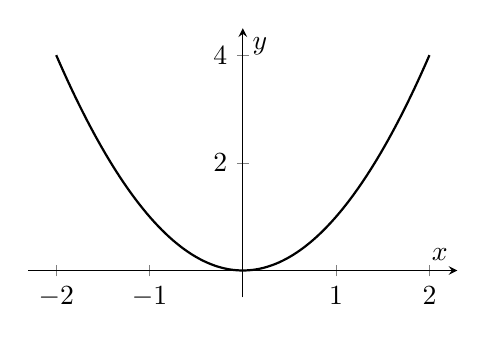
\begin{tikzpicture}
\begin{axis}[
    width=0.58\textwidth,
    height=5cm,
    axis lines=middle,
    xmin=-2.3,xmax=2.3,
    ymin=-0.5,ymax=4.5,
    xlabel={$x$},
    ylabel={$y$},
    samples=100
]
\addplot[thick,domain=-2:2]{x^2};
\end{axis}
\end{tikzpicture}
\end{center}

Thus a polynomial equation defines a geometric object.

Commutative algebra studies the algebraic structures that encode such
objects.

%%%%%%%%%%%%%%%%%%%%%%%%%%%%%%%%%%%%%%%%%%%%%%%%%%%%%%%%%%%%
\subsection{Vanishing Ideals}
\label{subsec:vanishing-ideals}
%%%%%%%%%%%%%%%%%%%%%%%%%%%%%%%%%%%%%%%%%%%%%%%%%%%%%%%%%%%%

Given a subset

\[ X\subseteq F^n, \]

one may consider all polynomials that vanish on \(X\):

\[ I(X)=\{f\in F[x_1,\ldots,x_n]:f(\vect{x})=0\text{ for every }\vect{x}\in X\}. \]

The set \(I(X)\) is an ideal.

Thus there are two fundamental constructions:

\[ I\longmapsto V(I) \]

and

\[ X\longmapsto I(X). \]

%%%%%%%%%%%%%%%%%%%%%%%%%%%%%%%%%%%%%%%%%%%%%%%%%%%%%%%%%%%%
\subsection{The Algebra--Geometry Correspondence}
\label{subsec:algebra-geometry-correspondence}
%%%%%%%%%%%%%%%%%%%%%%%%%%%%%%%%%%%%%%%%%%%%%%%%%%%%%%%%%%%%

\begin{center}
\begin{tikzpicture}[
    node distance=34mm,
    box/.style={draw,rounded corners,align=center,inner sep=7pt},
    >=stealth
]
\node[box] (ideals) {Ideals in\\\(F[x_1,\ldots,x_n]\)};
\node[box,right=of ideals] (sets) {Algebraic subsets\\of \(F^n\)};

\draw[->,thick,bend left=18] (ideals) to node[above]{\(I\mapsto V(I)\)}(sets);
\draw[->,thick,bend left=18] (sets) to node[below]{\(X\mapsto I(X)\)}(ideals);
\end{tikzpicture}
\end{center}

This relationship is developed much further in algebraic geometry.

%%%%%%%%%%%%%%%%%%%%%%%%%%%%%%%%%%%%%%%%%%%%%%%%%%%%%%%%%%%%
\subsection{Hilbert's Nullstellensatz}
\label{subsec:nullstellensatz-preview}
%%%%%%%%%%%%%%%%%%%%%%%%%%%%%%%%%%%%%%%%%%%%%%%%%%%%%%%%%%%%

Over an algebraically closed field, the relationship between ideals and
algebraic sets becomes particularly strong.

\begin{theorem}[Hilbert's Nullstellensatz --- Geometric Form]
Let \(F\) be algebraically closed and
\[ I\trianglelefteq F[x_1,\ldots,x_n]. \]
Then
\[ I(V(I))=\sqrt{I}. \]
\end{theorem}

The German word \emph{Nullstellensatz} is commonly translated as
``zero-locus theorem'' or ``theorem of zeros.''

This theorem explains why radical ideals are natural algebraic objects when
studying polynomial zero sets.

%%%%%%%%%%%%%%%%%%%%%%%%%%%%%%%%%%%%%%%%%%%%%%%%%%%%%%%%%%%%
\subsection{Why Radicals Appear Geometrically}
\label{subsec:why-radicals-geometric}
%%%%%%%%%%%%%%%%%%%%%%%%%%%%%%%%%%%%%%%%%%%%%%%%%%%%%%%%%%%%

Suppose

\[ f^n(\vect{x})=0. \]

Over a field,

\[ f(\vect{x})=0. \]

Therefore \(f\) and \(f^n\) have the same zero set.

For example,

\[ V(x)=V(x^2)=V(x^{100}). \]

Geometry cannot distinguish these powers through their zero sets alone.

This is why passing from an ideal \(I\) to its radical

\[ \sqrt{I} \]

preserves the same algebraic set.

%%%%%%%%%%%%%%%%%%%%%%%%%%%%%%%%%%%%%%%%%%%%%%%%%%%%%%%%%%%%
\subsection{Prime Ideal Chains}
\label{subsec:prime-ideal-chains}
%%%%%%%%%%%%%%%%%%%%%%%%%%%%%%%%%%%%%%%%%%%%%%%%%%%%%%%%%%%%

Prime ideals may form strictly increasing chains

\[ \mathfrak p_0\subsetneq\mathfrak p_1\subsetneq\cdots\subsetneq\mathfrak p_n. \]

The length of such chains measures an important notion of algebraic
dimension.

%%%%%%%%%%%%%%%%%%%%%%%%%%%%%%%%%%%%%%%%%%%%%%%%%%%%%%%%%%%%
\subsection{Krull Dimension}
\label{subsec:krull-dimension}
%%%%%%%%%%%%%%%%%%%%%%%%%%%%%%%%%%%%%%%%%%%%%%%%%%%%%%%%%%%%

\begin{definitionbox}{Krull Dimension}
The \emph{Krull dimension} of a commutative ring \(R\), denoted
\[ \dim(R), \]
is the supremum of the lengths of chains of prime ideals
\[ \mathfrak p_0\subsetneq\mathfrak p_1\subsetneq\cdots\subsetneq\mathfrak p_n. \]
\end{definitionbox}

The notation

\[ \dim(R) \]

is read ``the dimension of \(R\).''

%%%%%%%%%%%%%%%%%%%%%%%%%%%%%%%%%%%%%%%%%%%%%%%%%%%%%%%%%%%%
\subsection{Visualizing Krull Dimension}
\label{subsec:krull-dimension-visual}
%%%%%%%%%%%%%%%%%%%%%%%%%%%%%%%%%%%%%%%%%%%%%%%%%%%%%%%%%%%%

\begin{center}
\begin{tikzpicture}[
    node distance=10mm,
    box/.style={draw,rounded corners,minimum width=27mm,inner sep=5pt},
    >=stealth
]
\node[box] (p3) {\(\mathfrak p_3\)};
\node[box,below=of p3] (p2) {\(\mathfrak p_2\)};
\node[box,below=of p2] (p1) {\(\mathfrak p_1\)};
\node[box,below=of p1] (p0) {\(\mathfrak p_0\)};

\draw[->,thick] (p0)--node[right]{\(\subsetneq\)}(p1);
\draw[->,thick] (p1)--node[right]{\(\subsetneq\)}(p2);
\draw[->,thick] (p2)--node[right]{\(\subsetneq\)}(p3);

\node[right=12mm of p1,align=left] {chain length \(=3\)};
\end{tikzpicture}
\end{center}

Longer chains indicate greater algebraic dimension.

%%%%%%%%%%%%%%%%%%%%%%%%%%%%%%%%%%%%%%%%%%%%%%%%%%%%%%%%%%%%
\subsection{Examples of Krull Dimension}
\label{subsec:krull-dimension-examples}
%%%%%%%%%%%%%%%%%%%%%%%%%%%%%%%%%%%%%%%%%%%%%%%%%%%%%%%%%%%%

A field \(F\) has only one prime ideal:

\[ (0). \]

Therefore,

\[ \dim(F)=0. \]

The integers satisfy

\[ (0)\subsetneq(p) \]

for every prime \(p\), and no longer prime chain exists.

Thus

\[ \dim(\Z)=1. \]

For a field \(F\),

\[ \dim(F[x_1,\ldots,x_n])=n. \]

This result establishes a deep connection between algebraic dimension and the
number of independent polynomial variables.

%%%%%%%%%%%%%%%%%%%%%%%%%%%%%%%%%%%%%%%%%%%%%%%%%%%%%%%%%%%%
\subsection{Primary Ideals}
\label{subsec:primary-ideals}
%%%%%%%%%%%%%%%%%%%%%%%%%%%%%%%%%%%%%%%%%%%%%%%%%%%%%%%%%%%%

Prime ideals can be generalized.

\begin{definitionbox}{Primary Ideal}
A proper ideal \(Q\subsetneq R\) is \emph{primary} if
\[ ab\in Q\text{ and }a\notin Q \]
implies
\[ b^n\in Q \]
for some positive integer \(n\).
\end{definitionbox}

Equivalently,

\[ ab\in Q\implies a\in Q\text{ or }b\in\sqrt{Q}. \]

%%%%%%%%%%%%%%%%%%%%%%%%%%%%%%%%%%%%%%%%%%%%%%%%%%%%%%%%%%%%
\subsection{Radical of a Primary Ideal}
\label{subsec:radical-primary}
%%%%%%%%%%%%%%%%%%%%%%%%%%%%%%%%%%%%%%%%%%%%%%%%%%%%%%%%%%%%

If \(Q\) is primary, then

\[ \sqrt{Q} \]

is a prime ideal.

If

\[ \sqrt{Q}=\mathfrak p, \]

then \(Q\) is called a \(\mathfrak p\)-primary ideal.

Thus primary ideals sit naturally underneath prime ideals.

%%%%%%%%%%%%%%%%%%%%%%%%%%%%%%%%%%%%%%%%%%%%%%%%%%%%%%%%%%%%
\subsection{Example of a Primary Ideal}
\label{subsec:primary-ideal-example}
%%%%%%%%%%%%%%%%%%%%%%%%%%%%%%%%%%%%%%%%%%%%%%%%%%%%%%%%%%%%

In \(\Z\), consider

\[ (p^n) \]

where \(p\) is prime.

Then

\[ \sqrt{(p^n)}=(p). \]

The ideal \((p^n)\) is \((p)\)-primary.

For example,

\[ (8)=(2^3) \]

is \((2)\)-primary.

%%%%%%%%%%%%%%%%%%%%%%%%%%%%%%%%%%%%%%%%%%%%%%%%%%%%%%%%%%%%
\subsection{Primary Decomposition}
\label{subsec:primary-decomposition}
%%%%%%%%%%%%%%%%%%%%%%%%%%%%%%%%%%%%%%%%%%%%%%%%%%%%%%%%%%%%

A complicated ideal can sometimes be expressed as an intersection of
primary ideals.

Schematically,

\[ I=Q_1\cap\cdots\cap Q_n. \]

This is called a \emph{primary decomposition}.

For Noetherian rings, a fundamental theorem guarantees such decompositions
for proper ideals.

\begin{theorem}[Lasker--Noether Theorem]
Every proper ideal in a Noetherian commutative ring admits a finite primary
decomposition.
\end{theorem}

%%%%%%%%%%%%%%%%%%%%%%%%%%%%%%%%%%%%%%%%%%%%%%%%%%%%%%%%%%%%
\subsection{Why Primary Decomposition Matters}
\label{subsec:why-primary-decomposition}
%%%%%%%%%%%%%%%%%%%%%%%%%%%%%%%%%%%%%%%%%%%%%%%%%%%%%%%%%%%%

Primary decomposition resembles factorization.

Instead of decomposing an integer into prime powers,

\[ 60=2^2\cdot3\cdot5, \]

one decomposes an ideal into primary components:

\[ I=Q_1\cap\cdots\cap Q_n. \]

\begin{center}
\begin{tikzpicture}[
    node distance=12mm and 13mm,
    box/.style={draw,rounded corners,align=center,inner sep=5pt},
    >=stealth
]
\node[box] (I) {Ideal \(I\)};
\node[box,below left=of I] (Q1) {\(Q_1\)};
\node[box,below=of I] (Q2) {\(Q_2\)};
\node[box,below right=of I] (Q3) {\(Q_3\)};

\draw[->,thick] (I)--(Q1);
\draw[->,thick] (I)--(Q2);
\draw[->,thick] (I)--(Q3);

\node[below=8mm of Q2] {\(I=Q_1\cap Q_2\cap Q_3\)};
\end{tikzpicture}
\end{center}

Each primary component captures a different part of the ideal's structure.

%%%%%%%%%%%%%%%%%%%%%%%%%%%%%%%%%%%%%%%%%%%%%%%%%%%%%%%%%%%%
\subsection{Modules over Noetherian Rings}
\label{subsec:modules-noetherian-rings}
%%%%%%%%%%%%%%%%%%%%%%%%%%%%%%%%%%%%%%%%%%%%%%%%%%%%%%%%%%%%

The Noetherian condition extends naturally from rings to modules, as
introduced in \cref{sec:module-theory}.

A major result is:

\begin{theorem}
Let \(R\) be a Noetherian ring and \(M\) a finitely generated \(R\)-module.
Then \(M\) is a Noetherian \(R\)-module.
\end{theorem}

Consequently, every submodule of \(M\) is finitely generated.

This makes finitely generated modules over Noetherian rings especially
manageable.

%%%%%%%%%%%%%%%%%%%%%%%%%%%%%%%%%%%%%%%%%%%%%%%%%%%%%%%%%%%%
\subsection{Exact Sequences and Finite Generation}
\label{subsec:exact-sequences-finite-generation}
%%%%%%%%%%%%%%%%%%%%%%%%%%%%%%%%%%%%%%%%%%%%%%%%%%%%%%%%%%%%

Suppose

\[ 0\to M'\to M\to M''\to0 \]

is a short exact sequence of \(R\)-modules.

Finite-generation properties can often be transferred through this sequence.

For example, if both \(M'\) and \(M''\) are finitely generated, then \(M\) is
finitely generated.

Exact sequences therefore provide a systematic way to build complicated
modules from simpler pieces.

%%%%%%%%%%%%%%%%%%%%%%%%%%%%%%%%%%%%%%%%%%%%%%%%%%%%%%%%%%%%
\subsection{Nakayama's Lemma}
\label{subsec:nakayama-lemma}
%%%%%%%%%%%%%%%%%%%%%%%%%%%%%%%%%%%%%%%%%%%%%%%%%%%%%%%%%%%%

One of the central tools of local commutative algebra is Nakayama's Lemma.

\begin{theorem}[Nakayama's Lemma]
Let \((R,\mathfrak m)\) be a local ring and let \(M\) be a finitely generated
\(R\)-module. If
\[ \mathfrak mM=M, \]
then
\[ M=0. \]
\end{theorem}

A commonly used equivalent form says that if

\[ M=N+\mathfrak mM, \]

then

\[ M=N. \]

%%%%%%%%%%%%%%%%%%%%%%%%%%%%%%%%%%%%%%%%%%%%%%%%%%%%%%%%%%%%
\subsection{Interpreting Nakayama's Lemma}
\label{subsec:interpreting-nakayama}
%%%%%%%%%%%%%%%%%%%%%%%%%%%%%%%%%%%%%%%%%%%%%%%%%%%%%%%%%%%%

Consider the quotient

\[ M/\mathfrak mM. \]

Because

\[ R/\mathfrak m \]

is a field, this quotient is a vector space over the residue field

\[ k=R/\mathfrak m. \]

Nakayama's Lemma allows information about this simpler vector space to
control the original module \(M\).

\begin{center}
\begin{tikzpicture}[
    node distance=12mm,
    box/.style={draw,rounded corners,align=center,inner sep=5pt},
    >=stealth
]
\node[box] (M) {Module \(M\)\\over local ring \(R\)};
\node[box,below=of M] (quot) {\(M/\mathfrak mM\)};
\node[box,below=of quot] (vec) {Vector space over\\\(k=R/\mathfrak m\)};

\draw[->,thick] (M)--node[right]{quotient}(quot);
\draw[->,thick] (quot)--(vec);
\end{tikzpicture}
\end{center}

This is an important example of reducing a ring-theoretic problem to linear
algebra.

%%%%%%%%%%%%%%%%%%%%%%%%%%%%%%%%%%%%%%%%%%%%%%%%%%%%%%%%%%%%
\subsection{Minimal Generating Sets and Nakayama}
\label{subsec:minimal-generators-nakayama}
%%%%%%%%%%%%%%%%%%%%%%%%%%%%%%%%%%%%%%%%%%%%%%%%%%%%%%%%%%%%

Let \((R,\mathfrak m)\) be local and \(M\) finitely generated.

A set

\[ m_1,\ldots,m_n \]

generates \(M\) if their residue classes generate

\[ M/\mathfrak mM \]

as a vector space over

\[ R/\mathfrak m. \]

Thus the minimal number of generators of \(M\) is related to

\[ \dim_{R/\mathfrak m}(M/\mathfrak mM). \]

This provides a powerful bridge between module theory and ordinary linear
algebra.

%%%%%%%%%%%%%%%%%%%%%%%%%%%%%%%%%%%%%%%%%%%%%%%%%%%%%%%%%%%%
\subsection{Zero Divisors on Modules}
\label{subsec:zero-divisors-modules}
%%%%%%%%%%%%%%%%%%%%%%%%%%%%%%%%%%%%%%%%%%%%%%%%%%%%%%%%%%%%

An element \(r\in R\) may act as a zero divisor on an \(R\)-module \(M\).

This occurs when there exists

\[ 0\neq m\in M \]

such that

\[ rm=0. \]

Such behavior is encoded by annihilator ideals and leads to the theory of
associated prime ideals.

%%%%%%%%%%%%%%%%%%%%%%%%%%%%%%%%%%%%%%%%%%%%%%%%%%%%%%%%%%%%
\subsection{Associated Prime Ideals}
\label{subsec:associated-primes}
%%%%%%%%%%%%%%%%%%%%%%%%%%%%%%%%%%%%%%%%%%%%%%%%%%%%%%%%%%%%

\begin{definitionbox}{Associated Prime}
Let \(M\) be an \(R\)-module. A prime ideal \(\mathfrak p\) is
\emph{associated to \(M\)} if
\[ \mathfrak p=\Ann_R(m) \]
for some \(m\in M\).
\end{definitionbox}

The collection of associated primes is denoted

\[ \operatorname{Ass}_R(M). \]

This notation is read ``the associated primes of \(M\) over \(R\).''

Associated primes identify important locations where the module exhibits
zero-divisor behavior.

%%%%%%%%%%%%%%%%%%%%%%%%%%%%%%%%%%%%%%%%%%%%%%%%%%%%%%%%%%%%
\subsection{Support of a Module}
\label{subsec:support-module}
%%%%%%%%%%%%%%%%%%%%%%%%%%%%%%%%%%%%%%%%%%%%%%%%%%%%%%%%%%%%

\begin{definitionbox}{Support of a Module}
Let \(M\) be an \(R\)-module. The \emph{support} of \(M\) is
\[ \operatorname{Supp}_R(M)
=\{\mathfrak p\in\Spec(R):M_{\mathfrak p}\neq0\}. \]
\end{definitionbox}

The notation

\[ \operatorname{Supp}_R(M) \]

is read ``the support of \(M\) over \(R\).''

The support records the prime ideals at which the module remains visible
after localization.

%%%%%%%%%%%%%%%%%%%%%%%%%%%%%%%%%%%%%%%%%%%%%%%%%%%%%%%%%%%%
\subsection{Visualizing Module Support}
\label{subsec:module-support-visual}
%%%%%%%%%%%%%%%%%%%%%%%%%%%%%%%%%%%%%%%%%%%%%%%%%%%%%%%%%%%%

\begin{center}
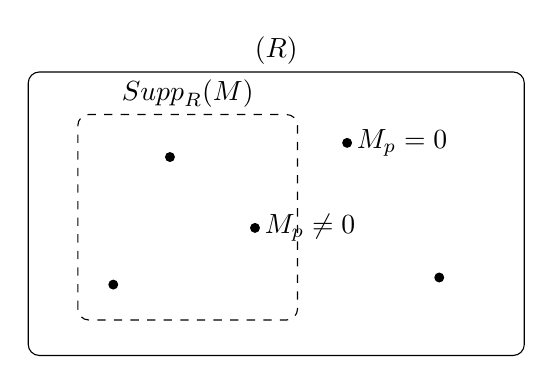
\begin{tikzpicture}[scale=0.9]
\draw[rounded corners] (0,0) rectangle (7,4);
\node at (3.5,4.3) {\(\Spec(R)\)};

\fill (1.2,1.0) circle (2pt);
\fill (2.0,2.8) circle (2pt);
\fill (3.2,1.8) circle (2pt);
\fill (4.5,3.0) circle (2pt);
\fill (5.8,1.1) circle (2pt);

\draw[dashed,rounded corners] (0.7,0.5) rectangle (3.8,3.4);
\node at (2.25,3.7) {\(\operatorname{Supp}_R(M)\)};

\node[right] at (4.5,3.0) {\(M_{\mathfrak p}=0\)};
\node[right] at (3.2,1.8) {\(M_{\mathfrak p}\neq0\)};
\end{tikzpicture}
\end{center}

The picture is schematic: points represent prime ideals rather than ordinary
Euclidean points.

%%%%%%%%%%%%%%%%%%%%%%%%%%%%%%%%%%%%%%%%%%%%%%%%%%%%%%%%%%%%
\subsection{The Zariski Topology: A Preview}
\label{subsec:zariski-topology-preview}
%%%%%%%%%%%%%%%%%%%%%%%%%%%%%%%%%%%%%%%%%%%%%%%%%%%%%%%%%%%%

The set

\[ \Spec(R) \]

can be equipped with a topology.

For an ideal \(I\trianglelefteq R\), define

\[ V(I)=\{\mathfrak p\in\Spec(R):I\subseteq\mathfrak p\}. \]

These sets are declared to be the closed sets of the \emph{Zariski topology}.

The term \emph{topology} will be developed canonically in
\cref{chap:topology}; here the construction is introduced only to reveal the
algebraic structure carried by \(\Spec(R)\).

%%%%%%%%%%%%%%%%%%%%%%%%%%%%%%%%%%%%%%%%%%%%%%%%%%%%%%%%%%%%
\subsection{Basic Closed Sets}
\label{subsec:basic-zariski-closed}
%%%%%%%%%%%%%%%%%%%%%%%%%%%%%%%%%%%%%%%%%%%%%%%%%%%%%%%%%%%%

For an element \(f\in R\), one often writes

\[ V(f)=V((f)). \]

This consists of all prime ideals containing \(f\):

\[ V(f)=\{\mathfrak p\in\Spec(R):f\in\mathfrak p\}. \]

If

\[ I=(f_1,\ldots,f_n), \]

then

\[ V(I)=V(f_1,\ldots,f_n). \]

%%%%%%%%%%%%%%%%%%%%%%%%%%%%%%%%%%%%%%%%%%%%%%%%%%%%%%%%%%%%
\subsection{Basic Open Sets}
\label{subsec:basic-zariski-open}
%%%%%%%%%%%%%%%%%%%%%%%%%%%%%%%%%%%%%%%%%%%%%%%%%%%%%%%%%%%%

The complement of \(V(f)\) is denoted

\[ D(f)=\Spec(R)\setminus V(f). \]

Therefore,

\[ D(f)=\{\mathfrak p\in\Spec(R):f\notin\mathfrak p\}. \]

The sets \(D(f)\) form a basis for the Zariski topology.

Localization at powers of \(f\),

\[ R_f, \]

is algebraically associated with the region \(D(f)\).

%%%%%%%%%%%%%%%%%%%%%%%%%%%%%%%%%%%%%%%%%%%%%%%%%%%%%%%%%%%%
\subsection{Localization and Geometry}
\label{subsec:localization-and-geometry}
%%%%%%%%%%%%%%%%%%%%%%%%%%%%%%%%%%%%%%%%%%%%%%%%%%%%%%%%%%%%

This produces an important algebra--geometry dictionary:

\begin{center}
\begin{tabularx}{0.9\textwidth}{@{}XX@{}}
\toprule
\textbf{Algebra} & \textbf{Geometric Interpretation}\\
\midrule
Prime ideal \(\mathfrak p\) & Point of \(\Spec(R)\)\\
Ideal \(I\) & Closed set \(V(I)\)\\
Localization \(R_{\mathfrak p}\) & Local behavior near a point\\
Localization \(R_f\) & Behavior on \(D(f)\)\\
Radical ideal & Geometric zero-set information\\
Krull dimension & Algebraic dimension\\
Module \(M\) & Algebraic data over the space\\
Support of \(M\) & Region where \(M\) is nonzero\\
\bottomrule
\end{tabularx}
\end{center}

This dictionary becomes foundational in algebraic geometry.

%%%%%%%%%%%%%%%%%%%%%%%%%%%%%%%%%%%%%%%%%%%%%%%%%%%%%%%%%%%%
\subsection{Worked Example: Localization}
\label{subsec:worked-localization}
%%%%%%%%%%%%%%%%%%%%%%%%%%%%%%%%%%%%%%%%%%%%%%%%%%%%%%%%%%%%

\begin{workedexamplebox}{Localization of \(\Z\) at \((5)\)}

Describe

\[ \Z_{(5)}. \]

\begin{tabularx}{\textwidth}{@{}>{\raggedright\arraybackslash}p{0.42\textwidth}X@{}}
Choose the prime ideal. & \(\mathfrak p=(5)\)\\
Take its complement. & \(S=\Z\setminus(5)\)\\
Determine allowed denominators. & Integers not divisible by \(5\)\\
Write the localization. &
\(\displaystyle \Z_{(5)}
=\left\{\frac{a}{b}\in\Q:5\nmid b\right\}\)
\end{tabularx}

\begin{answerbox}
\[ \boxed{\displaystyle
\Z_{(5)}
=\left\{\frac{a}{b}\in\Q:5\nmid b\right\}.} \]
\end{answerbox}
\end{workedexamplebox}

%%%%%%%%%%%%%%%%%%%%%%%%%%%%%%%%%%%%%%%%%%%%%%%%%%%%%%%%%%%%
\subsection{Worked Example: Radical of an Ideal}
\label{subsec:worked-radical}
%%%%%%%%%%%%%%%%%%%%%%%%%%%%%%%%%%%%%%%%%%%%%%%%%%%%%%%%%%%%

\begin{workedexamplebox}{Finding a Radical in \(\Z\)}

Find

\[ \sqrt{(72)}. \]

\begin{tabularx}{\textwidth}{@{}>{\raggedright\arraybackslash}p{0.42\textwidth}X@{}}
Factor the generator. & \(72=2^3\cdot3^2\)\\
Keep each distinct prime factor once. & \(2\cdot3=6\)\\
Form the corresponding ideal. & \(\sqrt{(72)}=(6)\)
\end{tabularx}

\begin{answerbox}
\[ \boxed{\sqrt{(72)}=(6).} \]
\end{answerbox}
\end{workedexamplebox}

%%%%%%%%%%%%%%%%%%%%%%%%%%%%%%%%%%%%%%%%%%%%%%%%%%%%%%%%%%%%
\subsection{Worked Example: Krull Dimension}
\label{subsec:worked-krull-dimension}
%%%%%%%%%%%%%%%%%%%%%%%%%%%%%%%%%%%%%%%%%%%%%%%%%%%%%%%%%%%%

\begin{workedexamplebox}{Dimension of a Polynomial Ring}

Determine the Krull dimension of

\[ F[x,y,z] \]

where \(F\) is a field.

\begin{tabularx}{\textwidth}{@{}>{\raggedright\arraybackslash}p{0.42\textwidth}X@{}}
Count the independent polynomial variables. & \(3\)\\
Use the polynomial-ring dimension theorem. & \(\dim(F[x_1,\ldots,x_n])=n\)\\
Substitute \(n=3\). & \(\dim(F[x,y,z])=3\)
\end{tabularx}

\begin{answerbox}
\[ \boxed{\dim(F[x,y,z])=3.} \]
\end{answerbox}
\end{workedexamplebox}

%%%%%%%%%%%%%%%%%%%%%%%%%%%%%%%%%%%%%%%%%%%%%%%%%%%%%%%%%%%%
\subsection{Common Errors in Commutative Algebra}
\label{subsec:commutative-algebra-errors}
%%%%%%%%%%%%%%%%%%%%%%%%%%%%%%%%%%%%%%%%%%%%%%%%%%%%%%%%%%%%

\subsubsection{Assuming Every Prime Ideal Is Maximal}

Every maximal ideal is prime, but the converse need not hold.

For example,

\[ (0)\subseteq\Z \]

is prime but not maximal.

%%%%%%%%%%%%%%%%%%%%%%%%%%%%%%%%%%%%%%%%%%%%%%%%%%%%%%%%%%%%
\subsubsection{Forgetting That Prime Ideals Are Proper}

The entire ring

\[ R \]

is never a prime ideal under the standard definition.

Likewise, maximal ideals must be proper.

%%%%%%%%%%%%%%%%%%%%%%%%%%%%%%%%%%%%%%%%%%%%%%%%%%%%%%%%%%%%
\subsubsection{Confusing Prime Elements with Prime Ideals}

A prime element \(p\) is an element of a ring.

A prime ideal \(\mathfrak p\) is a subset of a ring satisfying an ideal
condition.

In a suitable domain, a prime element may generate a prime ideal, but the
concepts are not identical.

%%%%%%%%%%%%%%%%%%%%%%%%%%%%%%%%%%%%%%%%%%%%%%%%%%%%%%%%%%%%
\subsubsection{Reversing Ideal Containment}

If

\[ a\mid b, \]

then

\[ (b)\subseteq(a), \]

not the other way around.

For example,

\[ 3\mid12 \]

but

\[ (12)\subseteq(3). \]

%%%%%%%%%%%%%%%%%%%%%%%%%%%%%%%%%%%%%%%%%%%%%%%%%%%%%%%%%%%%
\subsubsection{Treating Localization as Ordinary Fractions Without Care}

In an integral domain, localization behaves much like ordinary fractions.

In rings with zero divisors, equality of fractions requires the more general
equivalence relation.

%%%%%%%%%%%%%%%%%%%%%%%%%%%%%%%%%%%%%%%%%%%%%%%%%%%%%%%%%%%%
\subsubsection{Assuming Every Ring Is Noetherian}

Many important rings are Noetherian, but not every ring satisfies the
ascending chain condition.

For example, polynomial rings in infinitely many variables can fail to be
Noetherian.

%%%%%%%%%%%%%%%%%%%%%%%%%%%%%%%%%%%%%%%%%%%%%%%%%%%%%%%%%%%%
\subsubsection{Confusing Radical Ideals with Principal Square Roots}

The notation

\[ \sqrt{I} \]

does not mean taking numerical square roots of generators.

It means collecting all elements whose positive powers lie in \(I\).

%%%%%%%%%%%%%%%%%%%%%%%%%%%%%%%%%%%%%%%%%%%%%%%%%%%%%%%%%%%%
\subsubsection{Confusing Nilpotent and Zero-Divisor Elements}

Every nonzero nilpotent element is a zero divisor, but not every zero divisor
must be nilpotent.

%%%%%%%%%%%%%%%%%%%%%%%%%%%%%%%%%%%%%%%%%%%%%%%%%%%%%%%%%%%%
\subsubsection{Thinking \(\Spec(R)\) Contains Elements of \(R\)}

The points of

\[ \Spec(R) \]

are prime ideals, not ordinary ring elements.

%%%%%%%%%%%%%%%%%%%%%%%%%%%%%%%%%%%%%%%%%%%%%%%%%%%%%%%%%%%%
\subsubsection{Treating Krull Dimension as Vector-Space Dimension}

Krull dimension measures chains of prime ideals.

It is not defined by counting basis vectors.

%%%%%%%%%%%%%%%%%%%%%%%%%%%%%%%%%%%%%%%%%%%%%%%%%%%%%%%%%%%%
\subsection{Applications of Commutative Algebra}
\label{subsec:commutative-algebra-applications}
%%%%%%%%%%%%%%%%%%%%%%%%%%%%%%%%%%%%%%%%%%%%%%%%%%%%%%%%%%%%

\begin{applicationbox}
\textbf{Algebraic Geometry.}
Polynomial rings, ideals, prime spectra, localization, and dimension provide
the algebraic language used to study algebraic varieties and schemes.

\medskip

\textbf{Algebraic Number Theory.}
Integral extensions, integral closure, localization, prime ideals, and
Dedekind domains are used to study arithmetic beyond the ordinary integers.

\medskip

\textbf{Module Theory.}
Finitely generated modules over commutative rings encode linear-like
structures in settings where the scalars need not form a field.

\medskip

\textbf{Geometry.}
Local rings describe algebraic behavior near individual points, while Krull
dimension provides an algebraic notion corresponding to geometric dimension.

\medskip

\textbf{Polynomial Systems.}
Ideals encode systems of polynomial equations. Radical ideals preserve
zero-set information, and Noetherianity guarantees finite generation.

\medskip

\textbf{Topology.}
The prime spectrum of a ring carries the Zariski topology, converting
ring-theoretic information into a topological space.

\medskip

\textbf{Homological Algebra.}
Modules over commutative rings, exact sequences, localization, and
Noetherian conditions provide important settings for homological
constructions.
\end{applicationbox}

%%%%%%%%%%%%%%%%%%%%%%%%%%%%%%%%%%%%%%%%%%%%%%%%%%%%%%%%%%%%
\subsection{Structural Map of Commutative Algebra}
\label{subsec:commutative-algebra-map}
%%%%%%%%%%%%%%%%%%%%%%%%%%%%%%%%%%%%%%%%%%%%%%%%%%%%%%%%%%%%

\begin{center}
\begin{tikzpicture}[
    node distance=8mm and 12mm,
    box/.style={draw,rounded corners,align=center,inner sep=4pt,font=\small},
    >=stealth
]
\node[box] (rings) {Commutative rings};

\node[box,below left=of rings] (ideals) {Ideals};
\node[box,below right=of rings] (modules) {Modules};

\node[box,below left=of ideals] (prime) {Prime ideals};
\node[box,below right=of ideals] (radical) {Radicals};

\node[box,below left=of modules] (noeth) {Noetherian\\conditions};
\node[box,below right=of modules] (local) {Localization};

\node[box,below=24mm of rings] (spec) {\(\Spec(R)\)};
\node[box,below left=of spec] (dim) {Krull dimension};
\node[box,below right=of spec] (geom) {Algebraic geometry};

\draw[->] (rings)--(ideals);
\draw[->] (rings)--(modules);
\draw[->] (ideals)--(prime);
\draw[->] (ideals)--(radical);
\draw[->] (modules)--(noeth);
\draw[->] (modules)--(local);
\draw[->] (prime)--(spec);
\draw[->] (local)--(spec);
\draw[->] (spec)--(dim);
\draw[->] (spec)--(geom);
\end{tikzpicture}
\end{center}

%%%%%%%%%%%%%%%%%%%%%%%%%%%%%%%%%%%%%%%%%%%%%%%%%%%%%%%%%%%%
\subsection{Exercises}
\label{subsec:commutative-algebra-exercises}
%%%%%%%%%%%%%%%%%%%%%%%%%%%%%%%%%%%%%%%%%%%%%%%%%%%%%%%%%%%%

\begin{exercise}[1]
Explain why there is no distinction between left and right ideals in a
commutative ring.
\end{exercise}

\begin{exercise}[1]
Find the ideal
\[ (15,25)\subseteq\Z. \]
\end{exercise}

\begin{exercise}[1]
Find
\[ (18,30,42)\subseteq\Z. \]
\end{exercise}

\begin{exercise}[2]
Prove that the sum of two ideals is an ideal.
\end{exercise}

\begin{exercise}[2]
Prove that the product \(IJ\) of two ideals is an ideal.
\end{exercise}

\begin{exercise}[1]
Determine whether
\[ (7)\subseteq\Z \]
is prime.
\end{exercise}

\begin{exercise}[1]
Determine whether
\[ (7)\subseteq\Z \]
is maximal.
\end{exercise}

\begin{exercise}[1]
Determine whether
\[ (12)\subseteq\Z \]
is prime or maximal.
\end{exercise}

\begin{exercise}[2]
Prove that every maximal ideal of a commutative ring with identity is prime.
\end{exercise}

\begin{exercise}[2]
Prove that \(\mathfrak p\) is prime if and only if
\[ R/\mathfrak p \]
is an integral domain.
\end{exercise}

\begin{exercise}[2]
Prove that \(\mathfrak m\) is maximal if and only if
\[ R/\mathfrak m \]
is a field.
\end{exercise}

\begin{exercise}[1]
Find
\[ \sqrt{(36)}\subseteq\Z. \]
\end{exercise}

\begin{exercise}[1]
Find
\[ \sqrt{(200)}\subseteq\Z. \]
\end{exercise}

\begin{exercise}[2]
Show that every prime ideal is radical.
\end{exercise}

\begin{exercise}[2]
Determine the nilpotent elements of
\[ \Z/4\Z. \]
\end{exercise}

\begin{exercise}[2]
Determine the nilpotent elements of
\[ \Z/12\Z. \]
\end{exercise}

\begin{exercise}[1]
Explain why every integral domain is reduced.
\end{exercise}

\begin{exercise}[2]
Give an example of a reduced ring that is not an integral domain.
\end{exercise}

\begin{exercise}[1]
Explain why every field is Noetherian.
\end{exercise}

\begin{exercise}[1]
Explain why every PID is Noetherian.
\end{exercise}

\begin{exercise}[2]
State Hilbert's Basis Theorem and explain why it implies that
\[ F[x_1,\ldots,x_n] \]
is Noetherian.
\end{exercise}

\begin{exercise}[2]
Show that
\[ S=\{1,2,4,8,16,\ldots\}\subseteq\Z \]
is multiplicatively closed.
\end{exercise}

\begin{exercise}[1]
Describe the localization of \(\Z\) obtained by inverting every nonzero
integer.
\end{exercise}

\begin{exercise}[2]
Describe
\[ \Z_{(2)}. \]
Which rational numbers belong to this ring?
\end{exercise}

\begin{exercise}[2]
Determine whether each element belongs to \(\Z_{(3)}\):
\[ \frac12,\qquad\frac13,\qquad\frac57,\qquad\frac69. \]
\end{exercise}

\begin{exercise}[2]
Prove that \(R_{\mathfrak p}\) is a local ring for every prime ideal
\(\mathfrak p\).
\end{exercise}

\begin{exercise}[2]
Identify the unique maximal ideal of
\[ \Z_{(5)}. \]
\end{exercise}

\begin{exercise}[2]
Determine whether
\[ \sqrt{3} \]
is integral over \(\Z\).
\end{exercise}

\begin{exercise}[2]
Determine whether
\[ \frac12 \]
is integral over \(\Z\).
\end{exercise}

\begin{exercise}[2]
Show that every element of a finite field extension \(L/F\) is integral over
\(F\).
\end{exercise}

\begin{exercise}[1]
List the prime ideals of
\[ \Z/6\Z. \]
\end{exercise}

\begin{exercise}[1]
Describe
\[ \Spec(\Z). \]
\end{exercise}

\begin{exercise}[1]
Find
\[ \dim(F) \]
for a field \(F\).
\end{exercise}

\begin{exercise}[1]
Find
\[ \dim(F[x,y]). \]
\end{exercise}

\begin{exercise}[2]
Give a chain of prime ideals in \(F[x,y]\) of length \(2\).
\end{exercise}

\begin{exercise}[2]
Show that
\[ (p^n)\subseteq\Z \]
is \((p)\)-primary when \(p\) is prime.
\end{exercise}

\begin{exercise}[2]
Find the radical of
\[ (125)\subseteq\Z. \]
\end{exercise}

\begin{exercise}[2]
Explain the analogy between primary decomposition and prime-power
factorization of integers.
\end{exercise}

\begin{exercise}[2]
Let \((R,\mathfrak m)\) be local. Explain why
\[ R/\mathfrak m \]
is a field.
\end{exercise}

\begin{exercise}[3]
Let \(M\) be a finitely generated module over a local ring
\((R,\mathfrak m)\). Use Nakayama's Lemma to explain why
\[ M/\mathfrak mM=0 \]
implies
\[ M=0. \]
\end{exercise}

\begin{exercise}[2]
Let
\[ R=F[x,y]. \]
Describe the algebraic set
\[ V(x,y). \]
\end{exercise}

\begin{exercise}[2]
Sketch the real algebraic set
\[ V(y-x^2). \]
\end{exercise}

\begin{exercise}[2]
Explain why
\[ V(x)=V(x^4). \]
\end{exercise}

\begin{exercise}[2]
Show that
\[ V(I)=V(\sqrt{I}) \]
for ideals in a polynomial ring over a field.
\end{exercise}

\begin{exercise}[2]
For \(f\in R\), describe the basic open set
\[ D(f). \]
\end{exercise}

\begin{exercise}[2]
Explain why localization at \(f\) is naturally related to the basic open set
\[ D(f). \]
\end{exercise}

\begin{exercise}[2]
Define
\[ \operatorname{Supp}_R(M) \]
and explain its meaning using localization.
\end{exercise}

\begin{exercise}[3]
Explain how the following concepts fit together:
\[ \text{prime ideals},\quad\Spec(R),\quad\text{localization},\quad
\text{Krull dimension}. \]
\end{exercise}

%%%%%%%%%%%%%%%%%%%%%%%%%%%%%%%%%%%%%%%%%%%%%%%%%%%%%%%%%%%%
\subsection{Section Connections}
\label{subsec:commutative-algebra-connections}
%%%%%%%%%%%%%%%%%%%%%%%%%%%%%%%%%%%%%%%%%%%%%%%%%%%%%%%%%%%%

\chapterconnection{
Commutative algebra develops the structural theory of commutative rings
introduced in \cref{sec:ring-theory} and the module theory developed in
\cref{sec:module-theory}. Ideals become the central objects through which
quotients, prime spectra, radicals, localization, and dimension are studied.
Noetherian conditions guarantee finite algebraic descriptions, while
localization converts global problems into local ones. Prime ideals form the
points of \(\Spec(R)\), creating the fundamental bridge from algebra to
geometry. These ideas provide essential foundations for algebraic number
theory, algebraic geometry, homological algebra, and several later areas of
advanced mathematics.
}

%%%%%%%%%%%%%%%%%%%%%%%%%%%%%%%%%%%%%%%%%%%%%%%%%%%%%%%%%%%%
% SECTION SOURCE TRACKING
%%%%%%%%%%%%%%%%%%%%%%%%%%%%%%%%%%%%%%%%%%%%%%%%%%%%%%%%%%%%

%------------------------------------------------------------
% 1.9 Commutative Algebra
%------------------------------------------------------------
%
% Sources:
%   - M. F. Atiyah and I. G. Macdonald,
%     Introduction to Commutative Algebra.
%     Key: atiyahmacdonald1969commutative
%
% Used for:
%   - ideals, prime ideals, and maximal ideals;
%   - radicals and nilpotent elements;
%   - Noetherian rings and modules;
%   - localization of rings and modules;
%   - local rings;
%   - integral dependence and integral closure;
%   - prime spectra and dimension;
%   - primary ideals and primary decomposition;
%   - structural organization of introductory commutative algebra.
%
% Notes:
%   - Basic ring and ideal theory is treated canonically in Section 1.5.
%   - Module foundations are treated canonically in Section 1.8.
%   - The Zariski topology is introduced only as needed to explain Spec(R);
%     general topology belongs to Chapter 4.
%   - Algebraic sets and the Nullstellensatz are introduced as a bridge to
%     algebraic geometry; their geometric theory belongs to Section 3.8.
%   - Exact sequences are used only at an introductory level; their general
%     theory belongs to Section 1.13, Homological Algebra.
%   - Visualizations and pedagogical organization are independently
%     developed for this text.
%
\nocite{atiyahmacdonald1969commutative}